\section{Actor-Critic Methods}
\raggedbottom 
Many different approaches to different kind of reinforcement learning problems exist. 
Dynamic programming methods can compute optimal policies, however a perfect model of the environment as MDP is required.
Monte-Carlo methods on the other hand can estimate value functions and discover optimal policies by averaging over sampled trajectories.

\subsection{Monte-Carlo Predictions}

We call a complete run of the environment from start to termination an \textit{episode}.
Monte-Carlo predictions learn from complete episodes. They can be used to estimate the value of a state by calculating the discounted returns for every encountered state and changing the estimated value of the states slightly in the direction of the discounted return.

MC-methods learn relatively fast, however each update requires a full episode.

\subsection{TD-Learning}

\cite{Sut98} describes \textit{temporal difference} (TD) learning as one of the central ideas in reinforcement learning.
TD learning combines dynamic programming and Monte-Carlo ideas to learn eather \textit{state-values: V(s)} or \textit{state-action values: Q(s, a)}
Just like Monte-Carlo methods, TD-learning can learn directly from experience, while being able to learn without the need of finishing an episode through bootstrapping.

We will take a look at the most basic TD method for learning a value function. 
The update step is given as:

\begin{equation}
V(s_t)\gets V(s_t)+ \alpha [r_{t+1} + \gamma V(s_{t+1})-V(s_t)]
\end{equation}

Another popular TD-Method is Q-Learning.
It is used to estimate the state-action value function $Q$, and has a similar update step:

\begin{equation}
Q(s_t,a_t)\gets Q(s_t,a_t)+ \alpha [r_{t+1} + \gamma \max_a Q(s_{t+1},a)-Q(s_t,a_t)]
\end{equation}

After learning a Q-function, the agent has a reliable method to estimate and maximize the return, considering the learned function resembles the \textit{true state-value function} $Q*$ close enough. 
A common approach to achieve this is the use of a $\epsilon$-greedy policy, where a gradually decreasing value ($\epsilon$) is used to decide if a random action or the action assumed to be the best by the learned function is taken. This ensures both sufficient exploration and  exploitation, as it starts with a (mostly) random policy, and ends up with a deterministic policy always choosing the action with the highest estimated return.\citet{Sut98}

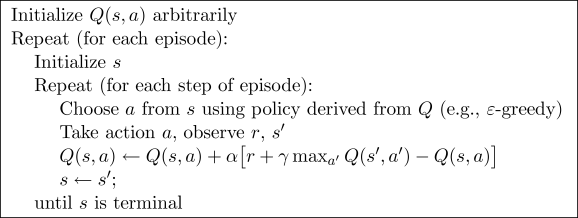
\includegraphics[scale=0.5]{bilder/qlearning2.png}

\caption{Q-learning algorithm taken from \citep{Sut98}}

\subsection{N-Step TD-Learning}

The TD-Learning algorithm shown only learns from a single step. Often episodes and be long, and the final reward (e.g. winning or losing a game) can be very important. 1-step learning can take a very long time to propagate this final reward into earlier states. In general TD-Learning is rather slow, compared to learning from full returns.

We can approach this problem by using n-step TD-learning.
Note that '$\inf$-step' TD update would be the same as a Monte-Carlo updates.

By combining the Monte-Carlo target
\begin{equation}
R_t = r_{t+1}+\gamma r_{t+2}+\gamma^2 r_{t+3}+\gamma^3 r_{t+4}++\gamma^T-t-1 r_{T}
\end{equation}

 ($T$ denotes the final step of the episode) with the TD approach, we can define the n-step TD-learning update:
 
\begin{equation}
V(s_t) = V(s_t) + \alpha(\gamma^nV(s_{t+n}+R_{t:t+n} - V(s_t)
\end{equation} 

where 

\begin{equation}
R_{t:t+n} = r_{t+1}+\gamma r_{t+2}+\gamma^2 r_{t+3}+ \dots +\gamma^{n-1} r_{t+n}
\end{equation}

denotes the discounted return for the next n steps.
\subsection{Critic-Only Methods}

The shown Q-learning algorith or SARSA are popular critic-only methods.

Critic-only methods learn state-action values. They do not contain an explicit function for the policy, but rather derive it from the learned state-action values by acting greedy on the Q-Values.

Critic-olny methods provice a low variance estimate of the expected returns, however the methods suffer from being biased and can be problematic in terms of convergence.

\subsection{Actor-Only Methods}

Onlike critic-only methods, actor only methods do not learn any state or state-action values.
Instead they perform optimization directly on the policy.
Usually a stochastic and parameterized policy $\pi_\theta$ is used.

Policy gradient methods like REINFORCE change the policy in order to maximize the average reward at a given timestep by performing gradient ascent. \citep{Williams1992}
We define an objective function $J(\theta)$ which is a measurement of performance.

The learning agent seeks to maximize $J(\theta)$ through gradient ascent

\begin{equation}
\theta_{t+1} = \theta_t + \alpha \widehat{\nabla J(\theta_t)}
\end{equation}

where $\widehat{\nabla J(\theta_t)}$ denotes an approximated gradient of the performance measure.
Methods of this schema are policy gradient methods \citep{Sut98} 

For the episodic case we define $J(\theta)$ to be the initial value of our policy. We should note that this only works under the assumption, that the environments always provides the same initial state.

\begin{equation}
J(\theta) \doteq v_{\pi_\theta}(s_0)
\end{equation}

We can approximate the gradient of $J(\theta)$ , $ \nabla v_{\pi_\theta}(s_0)$ through

\begin{equation}
\nabla J(\theta) \propto \sum_s \mu (s) \sum_a q_\pi (s,a) \nabla_\theta \pi(a \mid s, \theta)
\end{equation}

thanks to the policy gradient theorem. The proof for this theorem can be found in the reinforcement learning book by \citet{Sut98}.

$\mu$ denotes the on-policy distribution under $\pi$.

However if trajectories are sampled on-policy, we can simply rewrite this as the expectation under policy $\pi$:

\begin{equation}
\nabla J(\theta) \propto E_\pi \left[ \sum_a q_\pi (s_t,a) \nabla_\theta \pi (a \mid s_t, \theta) \right]
\end{equation}




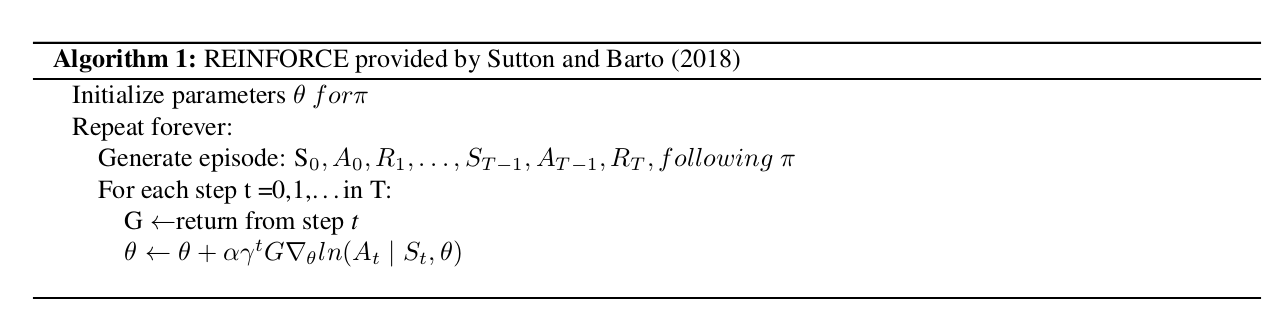
\includegraphics[scale=0.4]{bilder/REINFORCE.png}


In contrast to value based approaches, policy gradient methods provide strong convergence to at least a local maximum.
On top of that, actor methods are applicable on continuus action spaces.
 \citep{Sutton00policygradient}
 
Actor-only methods however suffer from a large variance of the gradient. Compared to critic-only methods their learning process is significantly slowed down. \citep{Grondman12}
 

\subsection{Actor-Critic Methods}

Actor-critic methods tackle the problem of high variance in policy gradient methods with the use of a critic.

They combine the strenght of both approaches to achieve a learning agent, which has strong convergence, yet low variance.

Since actor-critic methods are still policy gradient methods at their core, they provide the possibility to work on continuous actions spaces just like the actor-only approach.

The main reason for the variance in the gradient is the high variance of the return. By introducing a baseline $ b(s)$, to the objective function, we can achieve a lower variance, without creating bias.
The idea behind this is to increase the probability of an action in relation to how much better it is compared to other actions at this state, rather than the full return.

\begin{equation}
\nabla J(\theta) \propto \sum_s \mu(s) \left[ \left( \sum_a q_\pi (s,a) -b(s)\right) \nabla_\theta \pi (a \mid s, \theta) \right]
\end{equation}

The term $q_\pi(s_t,a) -b(s)$ can be replaced by different terms \citep{Schulman15}.
Popular choices for actor-critic learning are the advantage function $A_\pi$ (\ref{adv}) or the TD residual 

\begin{equation}
r_t + V_\pi(s_{t+1}) - V_\pi(s_t)
\end{equation} 



\begin{figure}
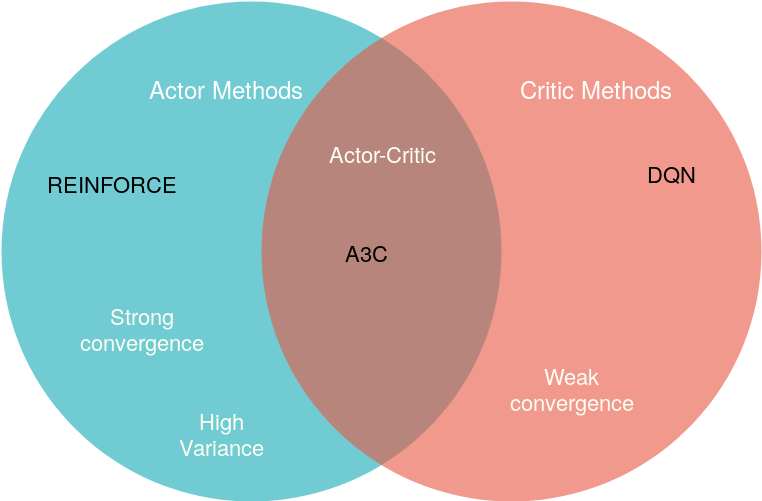
\includegraphics[scale=0.5]{bilder/actorcritic1.png}
\caption{Actor, Critic, and Actor-Critic approach}
\end{figure}

\pagebreak



\subsection{Asynchronous Advantage Actor Critic (A3C)}

In general we call an algorithm on policy, if the data used in the policy update was sampled under the same policy. The sequence of observed data encountered by an RL agent is strongly correlated and non-stationary \citep{A3C}. This can have a negative influence on the learning process.

Previous methods usually approached this problem by using randomly selected samples from a replay memory. \citep{mnih2015atari}

Training an agent comes with a high demand for computational power. To achieve feasible training times, former algorithms heavily relied on a strong GPU.

The asynchronous advantage actor critic(A3C) algorithm solves both problems, by training simultaneously on multiple environment.
Each learner samples trajectories and computes gradients. Those gradients are then applied to the shared parameters. 
After each global update step, the local parameters are synchronized.
This method not only enables efficient CPU computation with multiple threads, rather than requiring a strong GPU, but solves the problem of correlation since every environment can be assumed to be in different states.
Usually 16 or 32 environments are used, to ensure the decorrelation of the samples.

A3C samples trajectories of length $n$ and uses the longest possible k-return for the update step, meaning the last state uses a one-step update, the second to last a two-step update and so on, with the first state using an n-step update.
The gradients are accumulated over all state withing the trajectory and applied in a single gradient step. 

\begin{figure} 
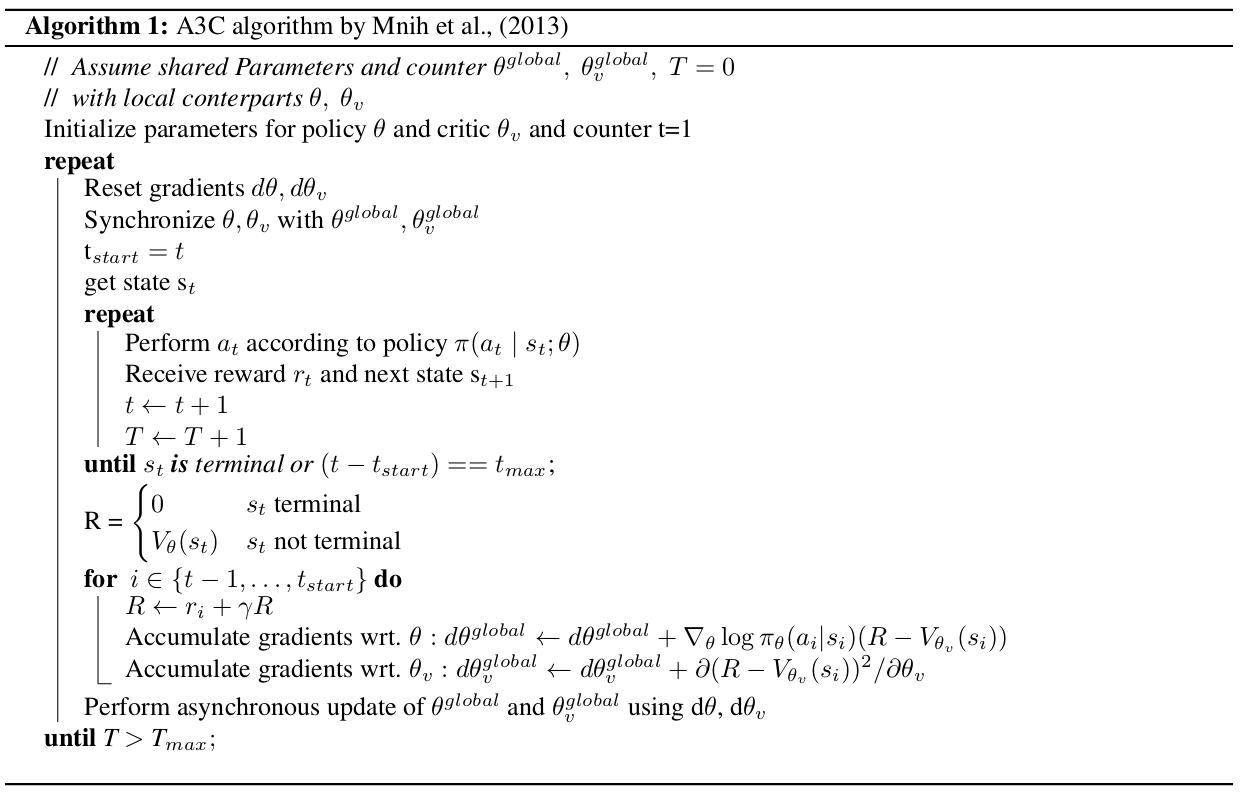
\includegraphics[scale=0.3]{bilder/aaac.png}
\caption{A3C by \citet{A3C}}
\end{figure}